\begin{figure}[H]
\centering

\begin{subfigure}{0.45\textwidth}
  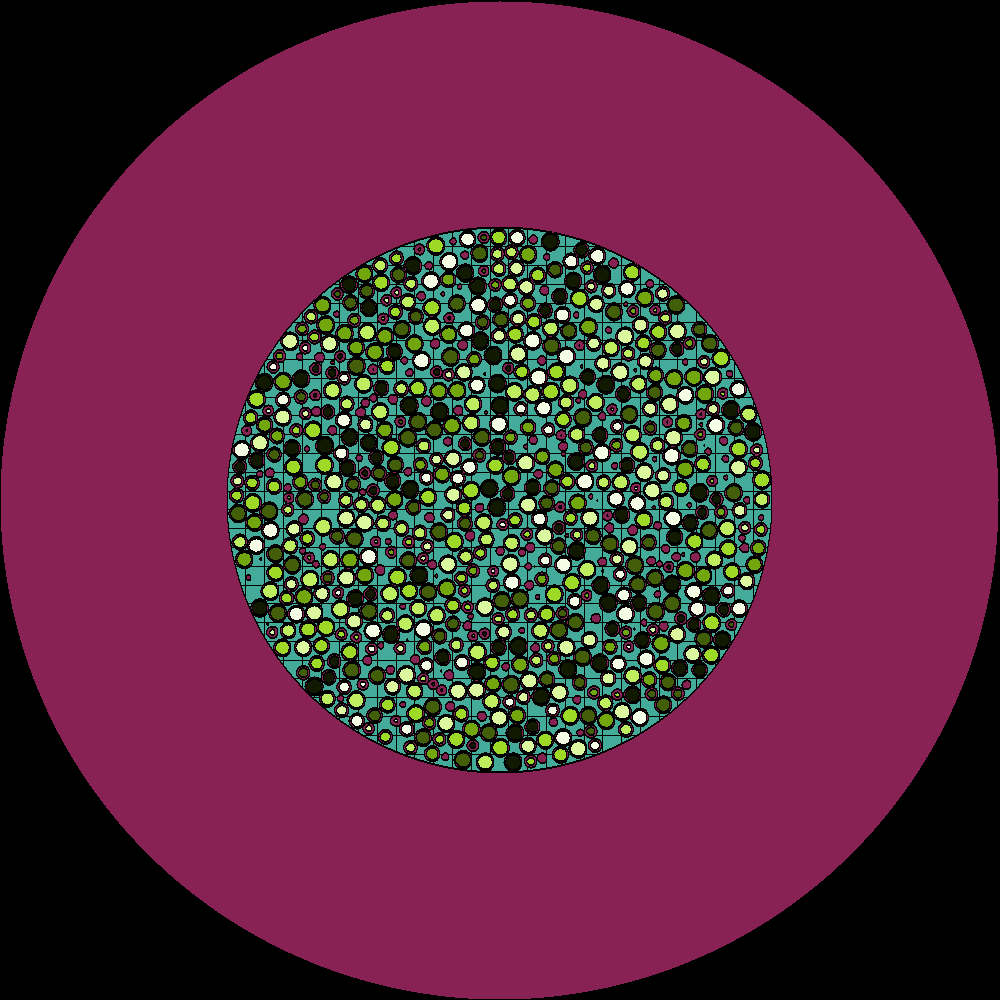
\includegraphics[width=0.95\linewidth]{figures/3456012/3456012-r}
  \caption{Radial Cross Section at y=0}
  \label{fig:3456012-r}
\end{subfigure}%
%
\begin{subfigure}{0.45\textwidth}
  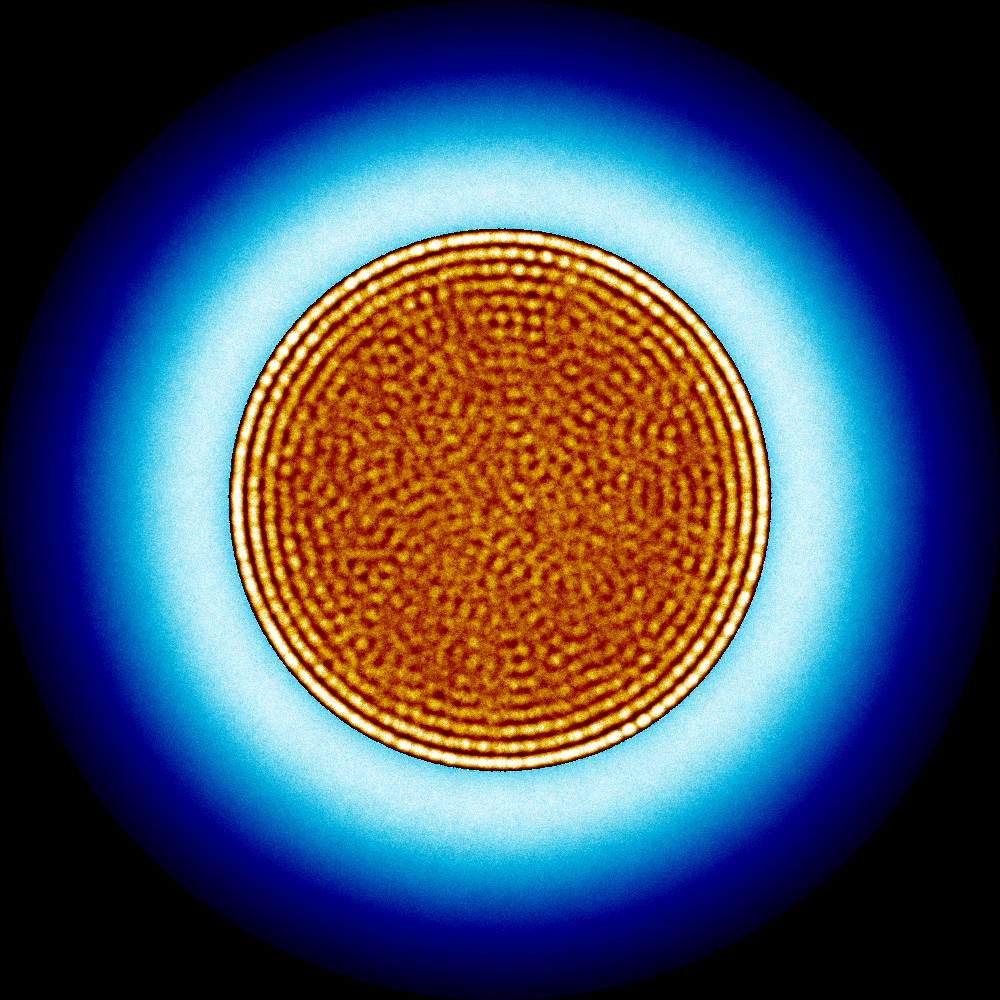
\includegraphics[width=0.95\linewidth]{figures/3456012/3456012-rm}
  \caption{Radial Mesh}
  \label{fig:3456012-rm}
\end{subfigure}

\begin{subfigure}{0.45\textwidth}
  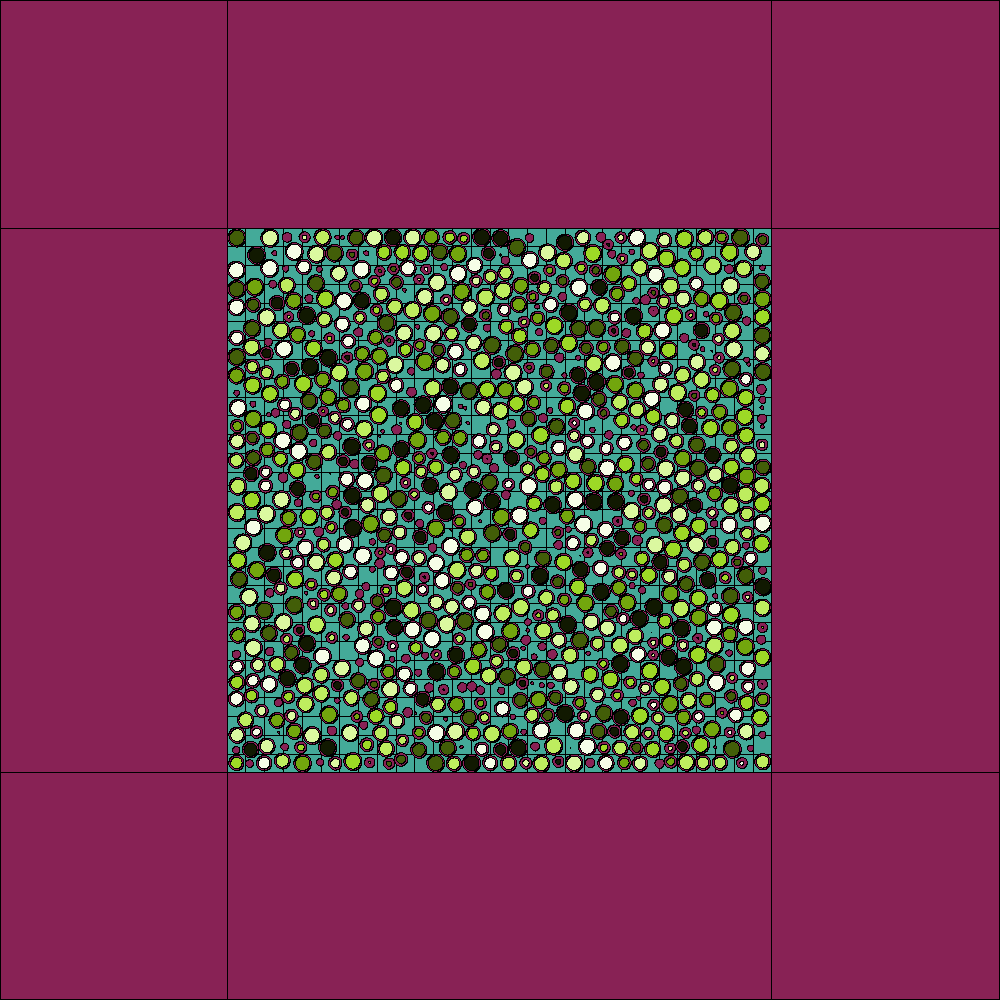
\includegraphics[width=0.95\linewidth]{figures/3456012/3456012-v}
  \caption{Axial Cross Section at z=0 }
  \label{fig:3456012-v}
\end{subfigure}
%
\begin{subfigure}{0.45\textwidth}
  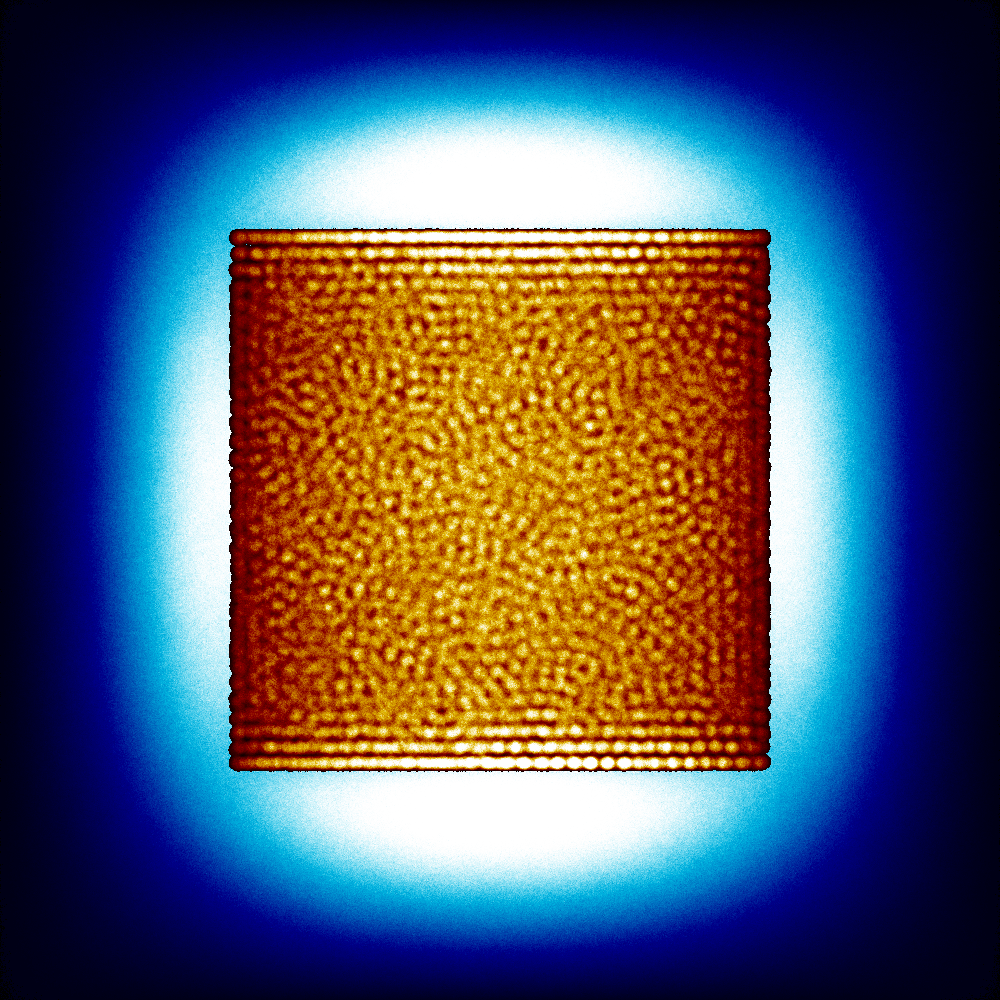
\includegraphics[width=0.95\linewidth]{figures/3456012/3456012-vm}
  \caption{Axial Mesh}
  \label{fig:3456012-vm}
\end{subfigure}
%
\caption{Shuffle Analysis: Run 3}
\label{fig:3456012}
\end{figure}